
\chapter{DISCUSÃO RESULTADOS} 

\par Este capítulo tem por finalidade representar e na integra o que foi
observado durante o desenvolvimento do trabalho e as dificuldades de pesquisa,
de desenvolvimento e diagramação.

\par Será inseridos também os dasafios que foram enfrentados para realização do
projeto.


\par De acordo com a pesquisa realizada o SNMP é essencial para o gerenciamento
de de redes, com foco no dispositivos que estejam conectados.

Segundo \citeonline{SNMP_Schmidt_Mauro}

\begin{citacao}
	O núcleo do SNMP é um conjunto simples de operaçãoes(e das informações obtidas
	por essas operações) que permitem ao administrador modificar o estado de alguns
	dispositivos baseados em SNMP. Por exemplo, é possível utilizar o SNMP para
	encerrar uma interfaceem roteador ou verificar a velocidade operacional de uma
	interface de Ethernet.
\end{citacao}


\par Devido ao grande volume de dados trafegados na rede, podemos assim complementa
que se faz necessário gerir a rede.

\par Segundo \citeonline{Java_Costa_Avancado}, atualmente identificamos o crescimento das redes, bem como
suas estruturas que possui infraestrura complexa. O aumento consideravél de acessos a rede
mundial de computadores á um incitamento impulsionando a criação de novos meios de manter
operantes as rede dentro das condições esperadas.

\par Para \citeonline{Redes_Mosharraf_Forouza},

\begin{citacao}
	Podemos definir o gerenciamento de redes como a tarefa de testar, monitorar,
	configurar e resolver problemas dos componentes de rede com o obejtivo
	de atender um conjunto de requisitos definidos por uma organização. Esses
	requisitos incluem a operação regular e eficiente de rede, proporcionando a
	qualidade de serviços predefinida para os usuários. Para realizar essa tarefa,
	um sistema de gerenciamento de rede usa hardware,software e seres humanos.(p.693).
\end{citacao}

\par Conforme \citeonline{Java_Costa_Avancado}, A adminstração de rede é fundamentada na coleta direta de
informação, que constitui toda a estrutura. Com base nesta informações podemos análisar uma
ou mais rede de forma dinâmica, fazendo-se compreender através de seu estado atual.

\par Para \citeonline{Projetos_Cabanis-brewin},
\begin{citacao}
	Documentos incluem planos, registros administrativos, dados técnicos, documentos
	de engenharia e construção, procedimentos, documentos sobre o sistema,
	relatórios e correspondências. Esta seção do plano de gerenciamento do
	projeto identifica os documentos que serão preparados no projeto e estabelece
	a abordagem administrativa, sistemas e procedimentos a serem utilizados para
	gerenciar essa documentação.(p.62)
\end{citacao}

\par A documentação é parte do trabalho, que formula os meios usados no decorrer do projeto,
facilitando a geração de relatórios e emplementação dos requisitos.

\par As imagens abaixo mostram como é a arquitetura utilizada na biblioteca
utilizada no java cujo é nomeada de snmpv4.



\begin{figure}[h!]
  \centerline{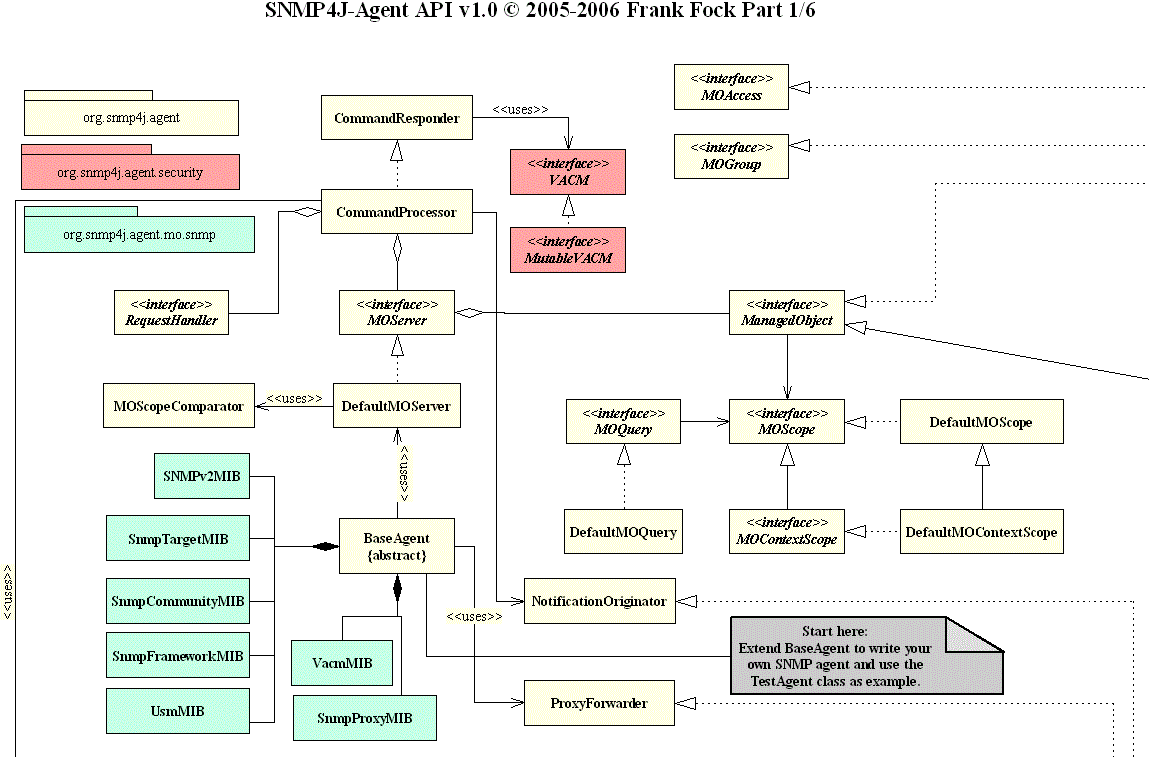
\includegraphics[scale=0.55]{./imagens/one.png}}
  \caption[Exemplo de criação de um projeto Web no Eclipse]
          {SNMP4J Client. \textbf{Fonte: snmp4j}
          \cite{Diagrama_do_SMNP4J}}
\label{fig:exemplo1}
\end{figure}





\begin{figure}[h!]
  \centerline{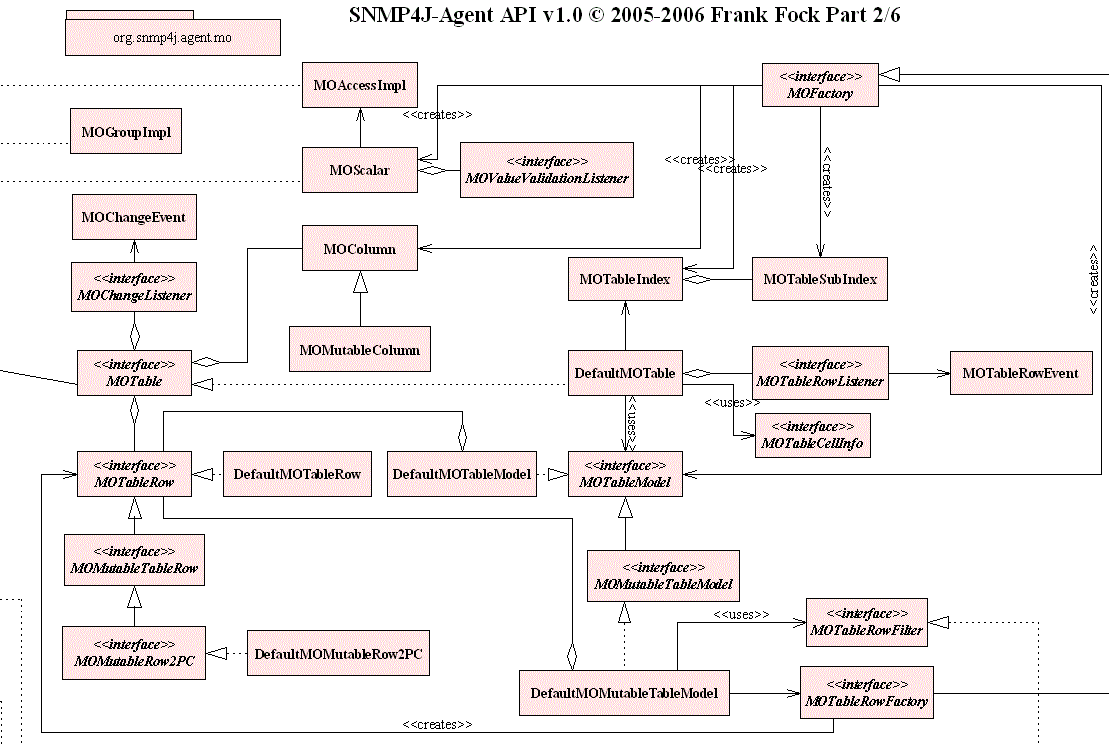
\includegraphics[scale=0.55]{./imagens/two.png}}
  \caption[Exemplo de criação de um projeto Web no Eclipse]
          {SNMP4J Client. \textbf{Fonte: snmp4j}
          \cite{Diagrama_do_SMNP4J}}
\label{fig:exemplo1}
\end{figure}




\begin{figure}[h!]
  \centerline{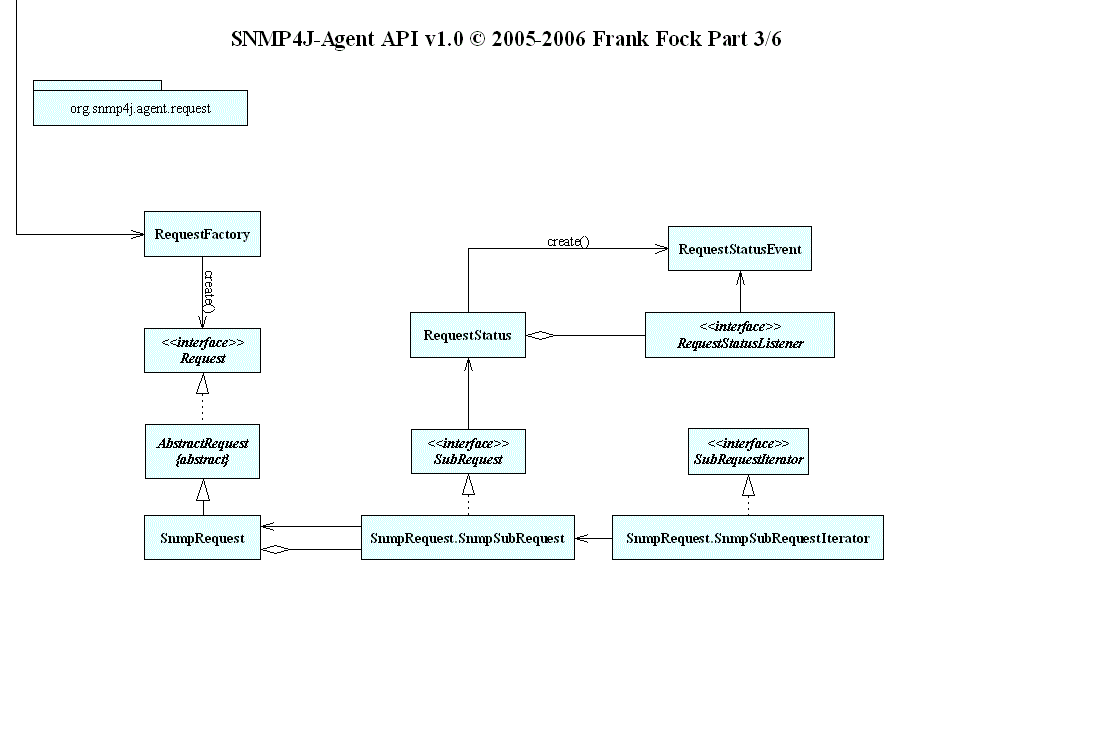
\includegraphics[scale=0.55]{./imagens/tres.png}}
  \caption[Exemplo de criação de um projeto Web no Eclipse]
          {SNMP4J Client. \textbf{Fonte: snmp4j}
          \cite{Diagrama_do_SMNP4J}}
\label{fig:exemplo1}
\end{figure}





\begin{figure}[h!]
  \centerline{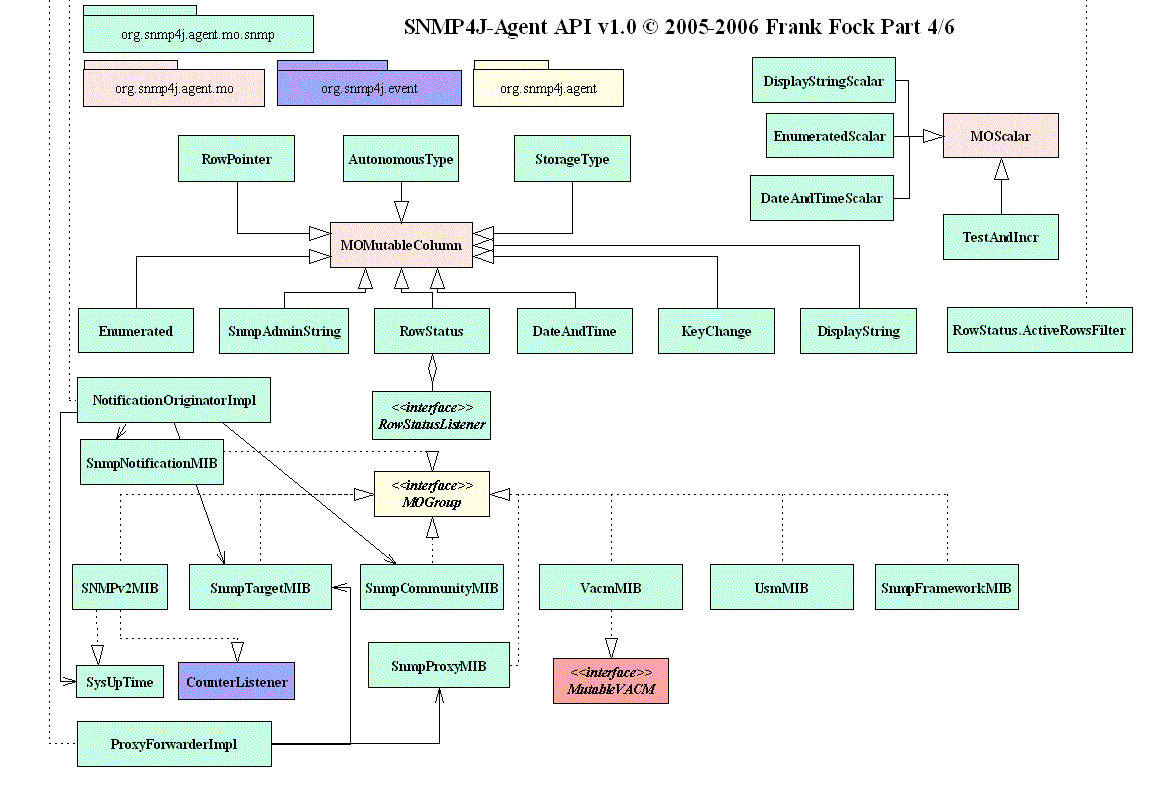
\includegraphics[scale=0.55]{./imagens/four.png}}
  \caption[Exemplo de criação de um projeto Web no Eclipse]
          {SNMP4J Client. \textbf{Fonte: snmp4j}
          \cite{Diagrama_do_SMNP4J}}
\label{fig:exemplo1}
\end{figure}




\begin{figure}[h!]
  \centerline{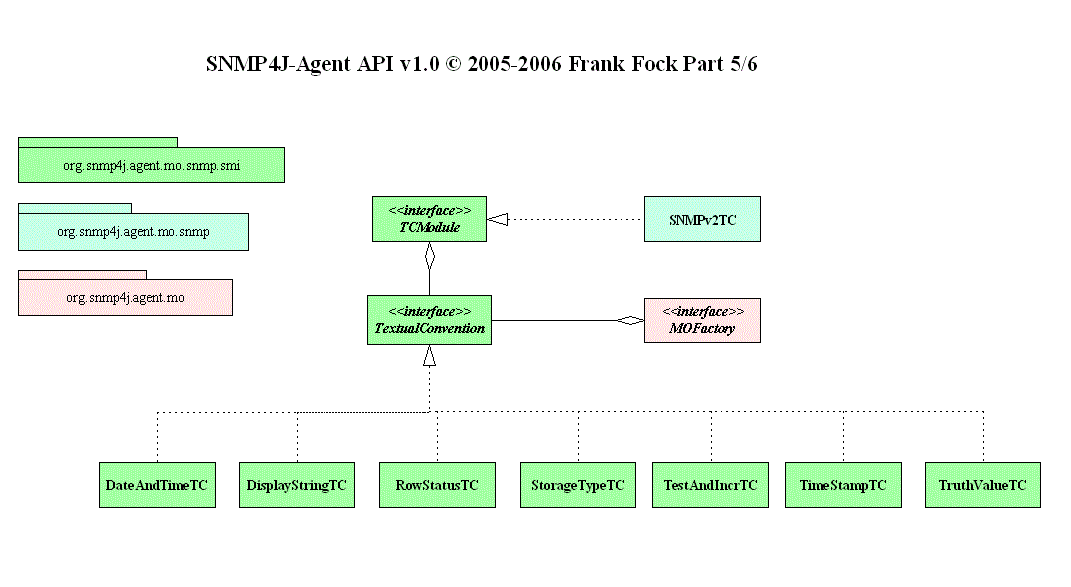
\includegraphics[scale=0.55]{./imagens/five.png}}
  \caption[Exemplo de criação de um projeto Web no Eclipse]
          {SNMP4J Client. \textbf{Fonte: snmp4j}
          \cite{Diagrama_do_SMNP4J}}
\label{fig:exemplo1}
\end{figure}



\begin{figure}[h!]
  \centerline{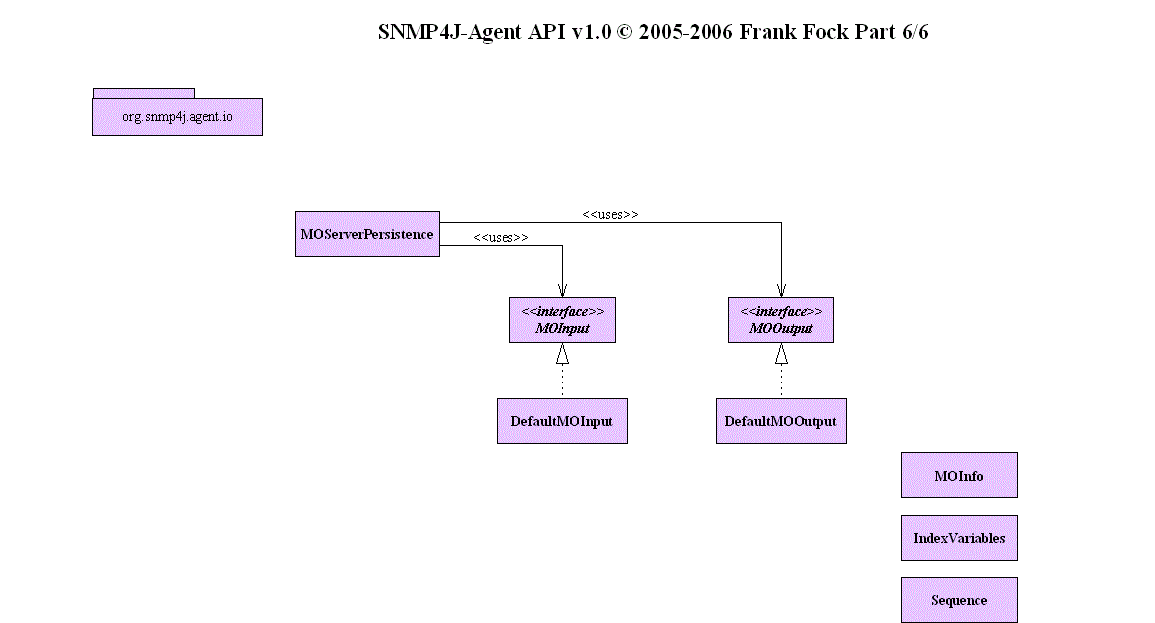
\includegraphics[scale=0.55]{./imagens/six.png}}
  \caption[Exemplo de criação de um projeto Web no Eclipse]
          {SNMP4J Client. \textbf{Fonte: snmp4j}
          \cite{Diagrama_do_SMNP4J}}
\label{fig:exemplo1}
\end{figure}


